\chapter{Caja y Egresos}
\label{mod:11-caja-y-egresos}

\section{Propósito}
\label{sec:caja-proposito}

Dos dominios estrechamente acoplados: \textbf{Caja} controla el efectivo físico por sucursal (apertura/cierre de sesión, arqueo) y registra todo movimiento de dinero (ingreso o egreso); \textbf{Egresos} modela las distintas formas en que el negocio gasta dinero (factura de proveedor, honorario profesional, gasto general, salario, factura de laboratorio) bajo una única jerarquía de datos.

\section{Entidades principales}
\label{sec:caja-entidades}

\begin{longtable}{p{6cm}p{9cm}}
\caption{Entidades principales del módulo de Caja y Egresos.}
\label{tab:caja-entidades}\\
\toprule
\textbf{Entidad} & \textbf{Rol} \\
\midrule
\endfirsthead
\toprule
\textbf{Entidad} & \textbf{Rol} \\
\midrule
\endhead
\bottomrule
\endfoot
\code{SesionCaja} & Una caja abierta por sucursal a la vez. Apertura con monto inicial, cierre con arqueo físico. \\
\code{MovimientoCaja} & Cada entrada/salida de dinero, siempre asociada a una \code{SesionCaja}; opcionalmente a una \code{Venta} (cobro) o un \code{Egreso} (pago). \\
\code{Egreso} (clase base TPH) & Ver \hyperref[adr:0011]{ADR 0011} --- una única tabla física \code{egresos}, discriminador \code{Tipo} (\code{TipoEgreso}). \\
\code{FacturaCompra} / \code{Honorario} / \code{GastoGeneral} / \code{SalarioEmpleado} / \code{Egreso}\allowbreak \code{Factura}\allowbreak \code{Laboratorio} & Los 5 subtipos concretos de \code{Egreso}. \\
\code{CategoriaGasto} & Catálogo para clasificar \code{GastoGeneral} (sin controller propio --- vive bajo \code{EgresosController}). \\
\end{longtable}

Ver el capítulo de Modelo de Datos (\S\ref{sec:modelo-datos}, Grupo C) para el diccionario de datos completo, y el \hyperref[adr:0011]{ADR 0011} para el razonamiento detrás de la herencia TPH.

\section{Reglas de negocio clave}
\label{sec:caja-reglas}

\begin{itemize}
  \item \textbf{Una sola \code{SesionCaja} abierta por sucursal a la vez} (\code{AbrirSesionAsync} rechaza si ya hay una \code{Abierta} o \code{Pendiente}\allowbreak \code{Aprobacion}). El monto de apertura, si no se especifica, se autocompleta con el \code{EfectivoContado} del último cierre de esa sucursal (el efectivo del cajón se traslada entre sesiones).
  \item \textbf{Cierre con tolerancia de arqueo:} al cerrar, se calcula \code{EfectivoEsperado = MontoInicial + ingresosEfectivo - egresosEfectivo} y se compara contra \code{EfectivoContado} (conteo físico). Si la diferencia está dentro de la tolerancia (\textpm\,50.000, fijada como constante \code{Tolerancia} en \code{CajaService}), la sesión pasa directo a \code{Cerrada}; si la excede, pasa a \code{Pendiente}\allowbreak \code{Aprobacion} y requiere que alguien con \code{aprobar_}\allowbreak \code{cierres_}\allowbreak \code{caja} la apruebe o la rechace. Rechazar \textbf{reabre} la sesión (vuelve a \code{Abierta}, limpiando los campos de cierre) para que el cajero pueda re-arquear.
  \item \textbf{\code{Egreso} centraliza sus propias transiciones de estado como métodos de dominio} (\code{egreso.}\allowbreak \code{RegistrarPago(.}\allowbreak \code{.}\allowbreak \code{.}\allowbreak \code{)}, \code{.Aprobar()}, \code{.Rechazar(motivo)}), no como lógica dispersa en el servicio --- lanzan \code{Invalid}\allowbreak \code{Operation}\allowbreak \code{Exception} si la transición no es válida en el estado actual, que el servicio traduce a \code{ErrorType.}\allowbreak \code{Conflict}.
  \item \textbf{Pago externo:} un egreso puede pagarse ``fuera de caja'' (\code{PagoExterno=true} + \code{MotivoPagoExterno} obligatorio) sin generar \code{MovimientoCaja} ni exigir sesión abierta --- para pagos que no pasaron por la caja física del negocio.
  \item Un egreso \textbf{pagado no se puede anular}; solo egresos en otros estados.
  \item \textbf{Dos caminos generan una \code{FacturaCompra}, no uno solo:} (a) \code{POST /api/egresos/facturas} (alta directa, sin OC) y (b) \code{ComprasService.}\allowbreak \code{RegistrarFacturaAsync} cuando la factura está ligada a una \code{PedidoProveedor} (ver Capítulo~\ref{mod:10-compras}). Ambos crean el mismo tipo de entidad \code{Egreso}/\code{FacturaCompra}, por caminos de código distintos.
  \item \textbf{El pago de un egreso registra el \code{MovimientoCaja} asociado} (\code{EgresoId = egreso.Id}) cuando el pago se hace vía \code{EgresoService.}\allowbreak \code{RegistrarPagoAsync}; el permiso que exige esta acción es \code{pagar_egresos}, definido a nivel de método en \code{EgresosController.}\allowbreak \code{RegistrarPago} (sobreescribe \code{gestionar_egresos} de la clase). El chequeo adicional de \code{aprobar_egresos} aplica solo para pago externo.
\end{itemize}

\section{Endpoints}
\label{sec:caja-endpoints}

Ver el Apéndice de Referencia de API § Caja y Egresos para la tabla completa (\code{CajaController}, \code{EgresosController}).

\begin{longtable}{p{1.3cm}p{7cm}p{6.3cm}}
\caption{Endpoints principales de Caja y Egresos.}
\label{tab:caja-endpoints}\\
\toprule
\textbf{Método} & \textbf{Ruta} & \textbf{Acción} \\
\midrule
\endfirsthead
\toprule
\textbf{Método} & \textbf{Ruta} & \textbf{Acción} \\
\midrule
\endhead
\bottomrule
\endfoot
POST & \code{/}\allowbreak \code{api/}\allowbreak \code{caja/}\allowbreak \code{sesiones} & Abrir sesión de caja \\
POST & \code{/}\allowbreak \code{api/}\allowbreak \code{caja/}\allowbreak \code{sesiones/}\allowbreak \code{{id}/cerrar} & Cerrar con arqueo $\to$ \code{Cerrada} o \code{Pendiente}\allowbreak \code{Aprobacion} \\
POST & \code{/}\allowbreak \code{api/}\allowbreak \code{caja/}\allowbreak \code{sesiones/}\allowbreak \code{{id}/aprobar-cierre} \textbar\ \code{rechazar-cierre} & Resolver una diferencia de arqueo \\
POST & \code{/}\allowbreak \code{api/}\allowbreak \code{egresos/}\allowbreak \texttt{\{facturas\textbar}\allowbreak \texttt{honorarios\textbar}\allowbreak \texttt{salarios\textbar}\allowbreak \texttt{gastos\}} & Crear el subtipo correspondiente de \code{Egreso} \\
PUT & \code{/api/egresos/{id}/pago} & Registrar pago (interno $\to$ \code{MovimientoCaja}, o externo) \\
PUT & \code{/api/egresos/{id}/}\allowbreak \code{{aprobar|rechazar|anular}} & Transiciones de estado \\
\end{longtable}

\section{Flujo típico}
\label{sec:caja-flujo}

El ciclo se muestra en dos figuras: creación y pago de un egreso (Figura~\ref{fig:seq-caja-egreso-pago}), y cierre de sesión con tolerancia de arqueo (Figura~\ref{fig:seq-caja-cierre}).

\begin{figure}[htbp]
\centering
% node distance corto: con 3.2cm la figura mide ~21cm y no entra en los
% 16cm de ancho de texto.
\begin{tikzpicture}[node distance=1.3cm]
  \node[actor] (c) {Cajero};
  \node[actor, right=of c] (sc) {SesionCaja};
  \node[actor, right=of sc] (eg) {Egreso};
  \node[actor, right=of eg] (mc) {Movimiento\\Caja};

  \draw[lineavida] (c.south) -- ++(0,-7.2);
  \draw[lineavida] (sc.south) -- ++(0,-7.2);
  \draw[lineavida] (eg.south) -- ++(0,-7.2);
  \draw[lineavida] (mc.south) -- ++(0,-7.2);

  \draw[mensaje] ($(c.south)+(0,-0.9)$) -- node[above,font=\scriptsize]{AbrirSesionAsync} node[below,font=\tiny\itshape]{Estado = Abierta} ($(sc.south)+(0,-0.9)$);
  \node[font=\tiny\itshape] at ($(eg)+(0,-2.1)$) {CrearXAsync (Estado = Pendiente)};
  \node[font=\tiny\itshape] at ($(eg)+(0,-2.9)$) {opt: AprobarEgresoAsync / RechazarEgresoAsync};
  \draw[mensaje] ($(c.south)+(0,-4.1)$) -- node[above,font=\scriptsize]{RegistrarPagoAsync} ($(eg.south)+(0,-4.1)$);
  \draw[mensaje] ($(eg.south)+(0,-5.3)$) -- node[above,font=\scriptsize,align=center]{(pago interno) exige SesionCaja Abierta} ($(sc.south)+(0,-5.3)$);
  \draw[mensaje] ($(eg.south)+(0,-6.3)$) -- node[above,font=\scriptsize,align=center]{(pago interno) crea MovimientoCaja\\(EgresoId = Eg.Id)} ($(mc.south)+(0,-6.3)$);
  \node[font=\tiny\itshape] at ($(eg)+(0,-7.0)$) {(pago externo) PagoExterno=true, sin MovimientoCaja};
\end{tikzpicture}
\caption{Apertura de sesión, creación de un egreso y registro de su pago (interno o externo). Tras el pago interno, el estado del egreso pasa a \texttt{Pagado}.}
\label{fig:seq-caja-egreso-pago}
\end{figure}

\begin{figure}[htbp]
\centering
\begin{tikzpicture}[node distance=3.4cm]
  \node[actor] (c) {Cajero};
  \node[actor, right=of c] (sc) {SesionCaja};
  \node[actor, right=of sc] (sup) {Supervisor};

  \draw[lineavida] (c.south) -- ++(0,-4.6);
  \draw[lineavida] (sc.south) -- ++(0,-4.6);
  \draw[lineavida] (sup.south) -- ++(0,-4.6);

  \draw[mensaje] ($(c.south)+(0,-0.9)$) -- node[above,font=\scriptsize]{CerrarSesionAsync (EfectivoContado)} ($(sc.south)+(0,-0.9)$);
  \node[font=\tiny\itshape] at ($(sc)+(0,-2.0)$) {diferencia dentro de tolerancia (\textpm\,50.000) $\to$ Estado = Cerrada};
  \node[font=\tiny\itshape] at ($(sc)+(0,-2.8)$) {diferencia fuera de tolerancia $\to$ Estado = PendienteAprobacion};
  \draw[mensaje] ($(sup.south)+(0,-4.0)$) -- node[above,font=\scriptsize,align=center]{AprobarCierreAsync / RechazarCierreAsync\\(rechazar reabre la sesión)} ($(sc.south)+(0,-4.0)$);
\end{tikzpicture}
\caption{Cierre de sesión con arqueo: dentro de tolerancia cierra directo, fuera de tolerancia requiere aprobación de un supervisor.}
\label{fig:seq-caja-cierre}
\end{figure}

\section{Vistas de frontend}
\label{sec:caja-frontend}

Rutas bajo \code{/caja/*} y \code{/egresos/*} (\code{SIGA-Web/}\allowbreak \code{src/}\allowbreak \code{router/}\allowbreak \code{index.}\allowbreak \code{ts}):

\begin{longtable}{p{5.2cm}p{4.2cm}p{3cm}}
\caption{Vistas de frontend del módulo Caja y Egresos.}
\label{tab:caja-vistas}\\
\toprule
\textbf{Vista} & \textbf{Ruta} & \textbf{Permiso} \\
\midrule
\endfirsthead
\toprule
\textbf{Vista} & \textbf{Ruta} & \textbf{Permiso} \\
\midrule
\endhead
\bottomrule
\endfoot
\code{CajaHistorialView.}\allowbreak \code{vue} & \code{/caja/historial} & \code{ver_ventas} \\
\code{CajaAprobacionesView.}\allowbreak \code{vue} & \code{/}\allowbreak \code{caja/}\allowbreak \code{aprobaciones} & \code{aprobar_}\allowbreak \code{cierres_}\allowbreak \code{caja} \\
\code{EgresosView.vue} & \code{/egresos} & \code{ver_egresos} \\
\code{NuevoEgresoView.}\allowbreak \code{vue} & \code{/egresos/nuevo} & \code{gestionar_}\allowbreak \code{egresos} \\
\code{AprobacionEgresosView.}\allowbreak \code{vue} & \code{/}\allowbreak \code{egresos/}\allowbreak \code{aprobacion} & \code{aprobar_egresos} \\
\code{PagosEgresosView.}\allowbreak \code{vue} / \code{PagoEgresoView.}\allowbreak \code{vue} & \code{/egresos/pagos}, \code{/}\allowbreak \code{egresos/}\allowbreak \code{pagos/}\allowbreak \code{:id} & \code{pagar_egresos} \\
\code{CategoriasGastoView.}\allowbreak \code{vue} & \code{/}\allowbreak \code{egresos/}\allowbreak \code{categorias} & \code{ver_egresos} \\
\end{longtable}

\section{Interfaz}
\label{sec:caja-interfaz}

\begin{figure}[htbp]
\centering
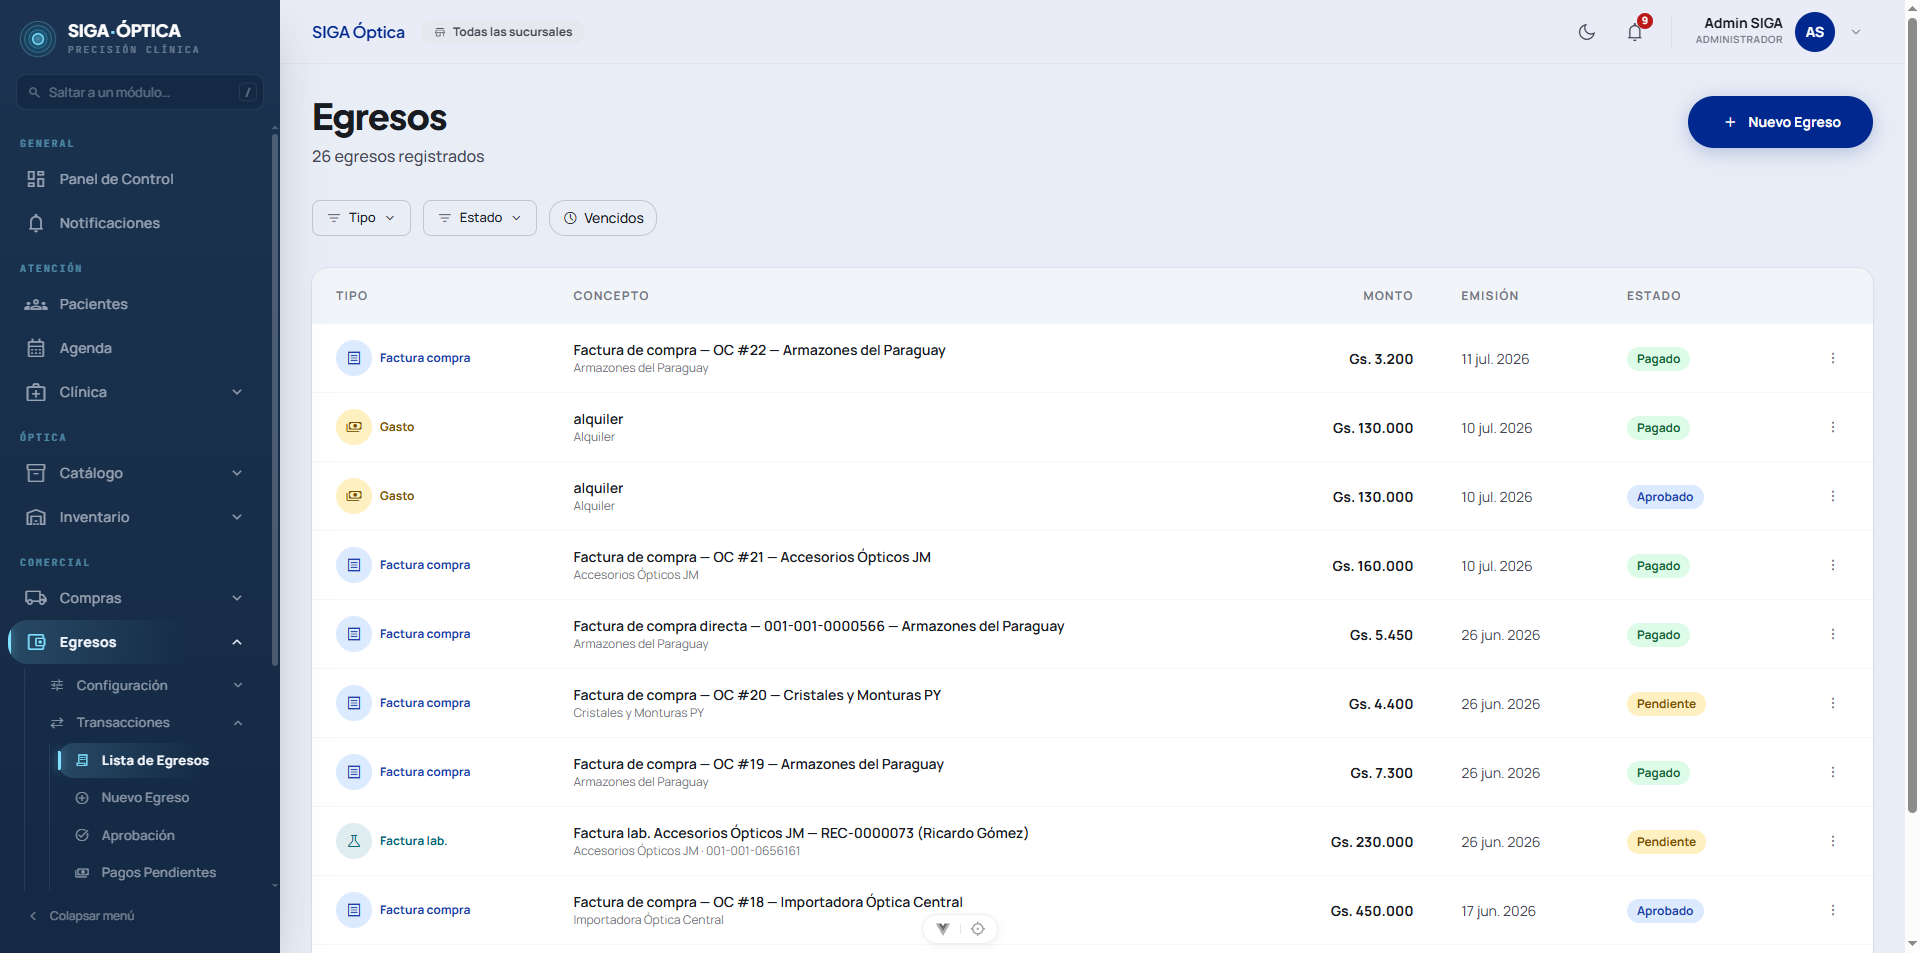
\includegraphics[width=0.95\textwidth]{imagenes/mod11-egresos.png}
\caption{Listado de egresos, agrupando facturas de compra, gastos generales y facturas de laboratorio.}
\label{fig:mod11-egresos}
\end{figure}

\section{Estado}
\label{sec:caja-estado}

\Implementado\ end-to-end.
